%%
%% This is file `sample-sigconf.tex',
%% generated with the docstrip utility.
%%
%% The original source files were:
%%
%% samples.dtx  (with options: `sigconf')
%% 
%% IMPORTANT NOTICE:
%% 
%% For the copyright see the source file.
%% 
%% Any modified versions of this file must be renamed
%% with new filenames distinct from sample-sigconf.tex.
%% 
%% For distribution of the original source see the terms
%% for copying and modification in the file samples.dtx.
%% 
%% This generated file may be distributed as long as the
%% original source files, as listed above, are part of the
%% same distribution. (The sources need not necessarily be
%% in the same archive or directory.)
%%
%%
%% Commands for TeXCount
%TC:macro \cite [option:text,text]
%TC:macro \citep [option:text,text]
%TC:macro \citet [option:text,text]
%TC:envir table 0 1
%TC:envir table* 0 1
%TC:envir tabular [ignore] word
%TC:envir displaymath 0 word
%TC:envir math 0 word
%TC:envir comment 0 0
%%
%%
%% The first command in your LaTeX source must be the \documentclass
%% command.
%%
%% For submission and review of your manuscript please change the
%% command to \documentclass[manuscript, screen, review]{acmart}.
%%
%% When submitting camera ready or to TAPS, please change the command
%% to \documentclass[sigconf]{acmart} or whichever template is required
%% for your publication.
%%
%%
\documentclass[sigconf]{acmart}
%\documentclass[journal=jacsat,manuscript=article]{achemso}

%\usepackage[sorting=none]{biblatex}
%\addbibresource{biblography.bib}
\usepackage{amsmath,amsfonts}
%\usepackage{algorithmic}
%\usepackage{algorithm}
\usepackage{algorithm2e}
%\usepackage{float}
\usepackage{graphicx}
\usepackage{textcomp}
\usepackage{multirow}
\usepackage{xcolor}
%\usepackage[normalem]{ulem}
\usepackage{cancel} %Note
\usepackage{multirow}
%\usepackage[normalem]{ulem}
% \useunder{\uline}{\ul}{}
%\usepackage{adjustbox}
\usepackage{tabularx}

%%
%% \BibTeX command to typeset BibTeX logo in the docs
\AtBeginDocument{%
  \providecommand\BibTeX{{%
    Bib\TeX}}}

%% Rights management information.  This information is sent to you
%% when you complete the rights form.  These commands have SAMPLE
%% values in them; it is your responsibility as an author to replace
%% the commands and values with those provided to you when you
%% complete the rights form.
\setcopyright{acmcopyright}
\copyrightyear{2024}
\acmYear{2024}
\setcopyright{acmlicensed}\acmConference[ICIIT 2024]{2024 9th International Conference on Intelligent Information Technology}{February 23--25, 2024}{Ho Chi Minh City, Vietnam}
\acmBooktitle{2024 9th International Conference on Intelligent Information Technology (ICIIT 2024), February 23--25, 2024, Ho Chi Minh City, Vietnam}
\acmDOI{10.1145/3654522.3654577}
\acmISBN{979-8-4007-1671-3/24/02}


%%
%% Submission ID.
%% Use this when submitting an article to a sponsored event. You'll
%% receive a unique submission ID from the organizers
%% of the event, and this ID should be used as the parameter to this command.
%%\acmSubmissionID{123-A56-BU3}

%%
%% For managing citations, it is recommended to use bibliography
%% files in BibTeX format.
%%
%% You can then either use BibTeX with the ACM-Reference-Format style,
%% or BibLaTeX with the acmnumeric or acmauthoryear sytles, that include
%% support for advanced citation of software artefact from the
%% biblatex-software package, also separately available on CTAN.
%%
%% Look at the sample-*-biblatex.tex files for templates showcasing
%% the biblatex styles.
%%

%%
%% The majority of ACM publications use numbered citations and
%% references.  The command \citestyle{authoryear} switches to the
%% "author year" style.
%%
%% If you are preparing content for an event
%% sponsored by ACM SIGGRAPH, you must use the "author year" style of
%% citations and references.
%% Uncommenting
%% the next command will enable that style.
%%\citestyle{acmauthoryear}


%%
%% end of the preamble, start of the body of the document source.




\begin{document}

%%
%% The "title" command has an optional parameter,
%% allowing the author to define a "short title" to be used in page headers.
\title{ChainSniper: A Machine Learning Approach for Auditing Cross-Chain Smart Contracts}

%%
%% The "author" command and its associated commands are used to define
%% the authors and their affiliations.
%% Of note is the shared affiliation of the first two authors, and the
%% "authornote" and "authornotemark" commands
%% used to denote shared contribution to the research.
\author{Tuan-Dung Tran}
%%\authornote{Both authors contributed equally to this research.}
\email{dungtran@uit.edu.vn}
\orcid{0000-0003-1156-7072}
%%\authornotemark[1]
\affiliation{%
  \institution{University of Information Technology, Vietnam National University}
  \city{Ho Chi Minh city}
  \country{Vietnam}
  \postcode{700000}
}

\author{Kiet Anh Vo}
\email{20520605@gm.uit.edu.vn}
\orcid{0009-0004-0883-1236}
\affiliation{%
  \institution{University of Information Technology, Vietnam National University}
  \city{Ho Chi Minh city}
  \country{Vietnam}
  \postcode{700000}
}

\author{Phan The Duy}
\email{duypt@uit.edu.vn}
\orcid{0000-0002-5945-3712}
%%\authornotemark[1]
\affiliation{%
  \institution{University of Information Technology, Vietnam National University}
  \city{Ho Chi Minh city}
  \country{Vietnam}
  \postcode{700000}
}

\author{Nguyen Tan Cam}
\email{camnt@uit.edu.vn}
\orcid{0000-0002-1489-2826}
\affiliation{%
  \institution{University of Information Technology, Vietnam National University}
  \city{Ho Chi Minh city}
  \country{Vietnam}
  \postcode{700000}
}

\author{Van-Hau Pham}
\email{haupv@uit.edu.vn}
\orcid{0000-0003-3147-3356}
\affiliation{%
  \institution{University of Information Technology, Vietnam National University}
  \city{Ho Chi Minh city}
  \country{Vietnam}
  \postcode{700000}
}
%%
%% By default, the full list of authors will be used in the page
%% headers. Often, this list is too long, and will overlap
%% other information printed in the page headers. This command allows
%% the author to define a more concise list
%% of authors' names for this purpose.
\renewcommand{\shortauthors}{TD. Tran et al.}

%%
%% The abstract is a short summary of the work to be presented in the
%% article.
\begin{abstract}
Smart contracts are autonomous programs stored on blockchain networks that self-execute agreed terms in a transparent and accurate manner. Within cross-chain platforms, smart contracts facilitate interaction and exchange of data between diverse blockchains. However, the presence of vulnerabilities in smart contracts renders them susceptible to exploitation, jeopardizing security. Considerable research has focused on identifying and detecting such vulnerabilities, though existing approaches have yet to achieve comprehensive coverage. This paper presents ChainSniper, a sidechain-based framework integrating machine learning to automatically appraise vulnerabilities in cross-chain smart contracts. A comprehensive dataset, denoted "CrossChainSentinel", was compiled comprising 300 manually labeled code snippets. This dataset was leveraged to train machine learning models discerning vulnerable versus secure smart contracts. Experimental findings demonstrate the viability of machine learning methodologies for enhancing smart contract auditing within decentralized applications spanning multiple networks. Notable detection precision was achieved, substantiating ChainSniper's potential to strengthen security analysis through an automated and expansive evaluation of smart contract code. 
%While prior work made strides, comprehensive solutions have remained elusive. ChainSniper aims to address this gap through a representative training corpus and specialized sidechain architecture facilitating broad vulnerability screening across interconnected blockchain platforms. Continued enlargement of the underlying dataset and model optimization are expected to further augment capabilities.
\end{abstract}

\ccsdesc[500]{Security and privacy~Distributed systems security}
\keywords{Cross-chain, Smart Contract, Vulnerability, Machine Learning}
\settopmatter{printfolios=true}
\maketitle

\section{Introduction}
% SUON VIET INTRODUCTION
% DOAN 1: Gioi thieu chung ve blockchain/crosschain, gom: 1-2 cau gioi thieu ve blockchain nhu dac diem&uu diem; gom 2-3 ve nhuoc diem cua no và cần nói được vấn đề cô lập/thiếu khả năng giao tiếp liên chuỗi trong multi blockchain; gom 3-4 cau gioi thieu cross-chain, câu cuối cần nổi bật crosschain solution SIDECHAIN (vì m làm trên cái này).
% DOAN 2: Vấn đề của cross-chain: Phân tích vai trò smart contract trong cross-chain và vul của SM, thêm các cite minh chứng cho việc smart contract bị tấn công (trong các hệ thống cross  -chain). xxx được thì nên thêm giải thích Vul của SM crosschain vs Vul của SM blockchain thường có gì khác nhau(khả năng khai thác, hậu quả, mức độ ảnh hưởng).
% DOAN 3: Cite các nghiên cứu hiện tại cho vấn đê nêu trên, nêu nhược điểm, làm bật lí do tại sao nên ứng dụng ML trong việc phát hiện lỗ hổng trong SM của cross-chain.
% DOAN 4: main contributions
The idea behind blockchain is to build a decentralized network that provides capabilities for storing, exchanging, and verifying data and most importantly, makes services and transactions on the network more reliable and authentic \cite{Patel_Patel_2023, Kumarathunga_Calheiros_Ginige_2022}. However, to have these powerful features, blockchain systems are often built independently with their own rules and protocols, leading to blockchains having no interoperability across chains. In order that, Cross-chain technology refers to a set of protocols and systems that enable interoperability and communication between multiple blockchain networks \cite{xie2022zkbridge}. Cross-chain technology aims to connect these isolated ecosystems, allowing assets and data to be transferred and shared seamlessly across various blockchains \cite{lan2021horizon}. This innovation is crucial in addressing the limitations of scalability, speed, and functionality that individual blockchains often face. By facilitating cross-chain communication, users can harness the advantages of different blockchains, enhance liquidity, and promote a more interconnected and efficient blockchain ecosystem. Different techniques like atomic swaps, wrapped tokens, sidechains, and decentralized bridges are used to allow interoperability between blockchain networks. This interoperability enables blockchain networks to work together seamlessly, moving toward a future where they can co-exist in harmony.

\begin{figure}[hbt]
  \centering
  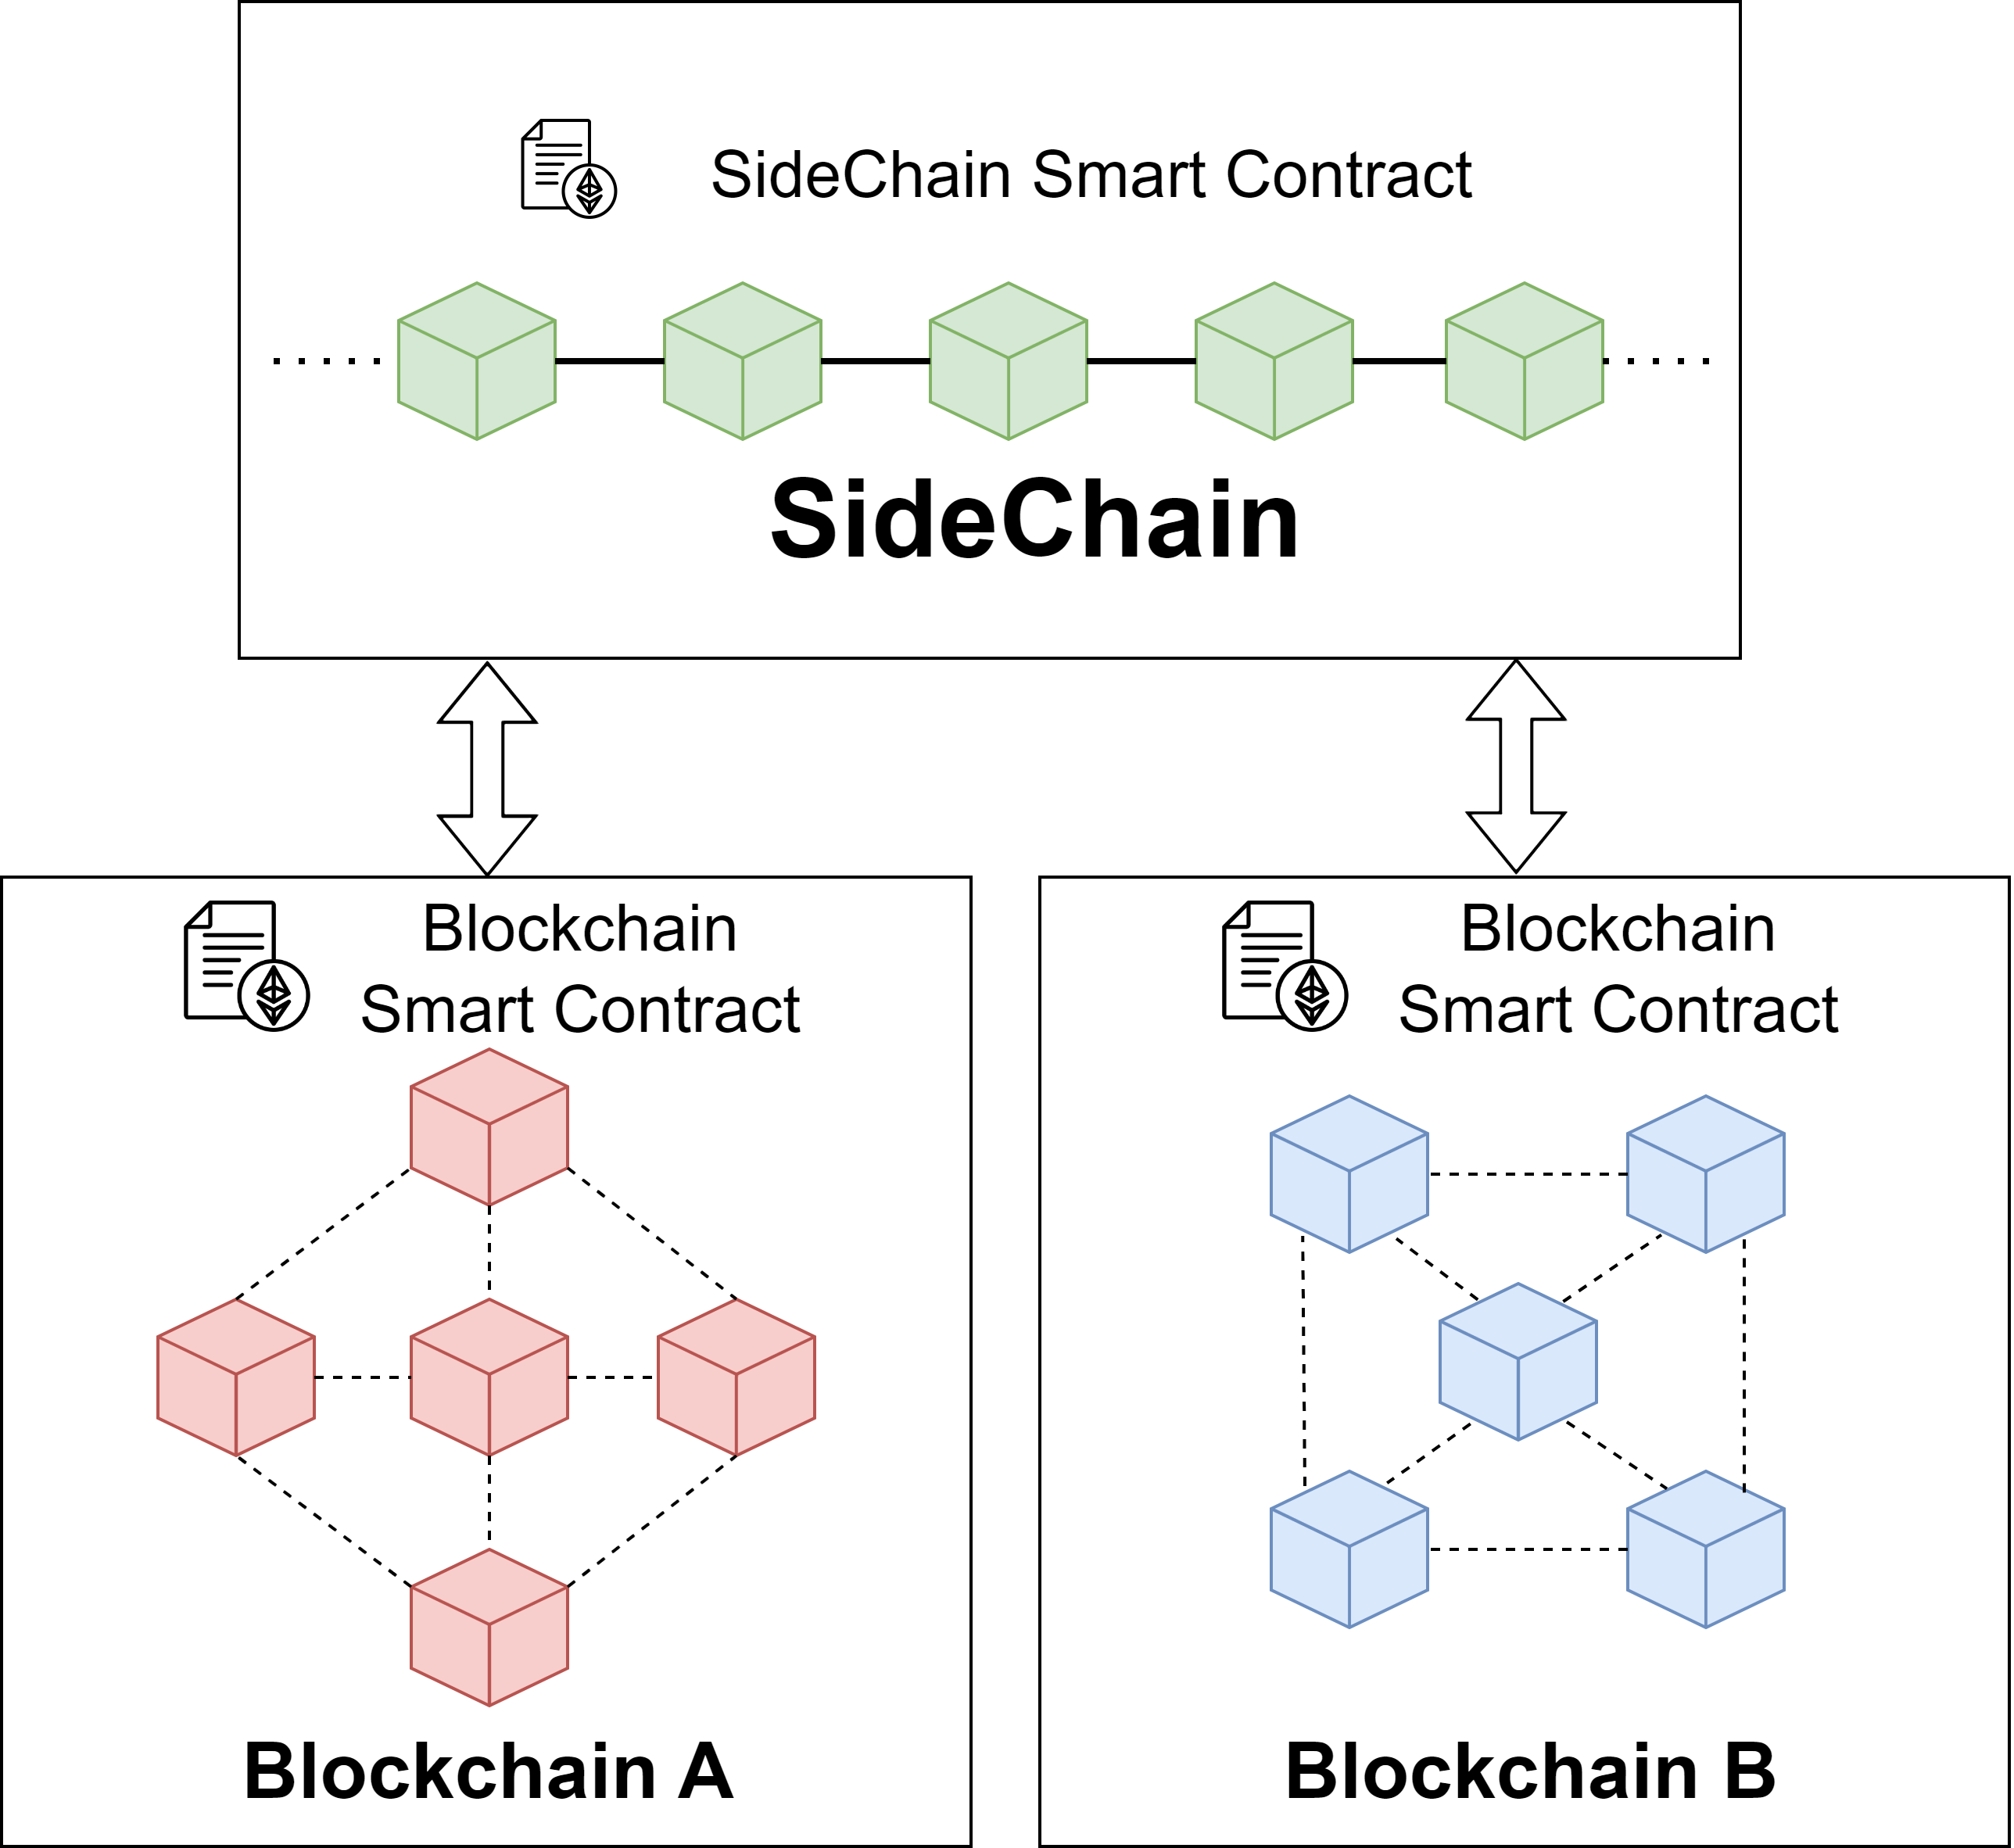
\includegraphics[width=0.9\linewidth]{SideChainMain.png}
  \caption{The interchain communication between two blockchains through a sidechain.}
  \Description{The concept of crosschain}
\end{figure}

%add thông tin về các cuộc tấn công lên mạng cross chain dựa trên thông  dựa trên
% đã add cuộc tấn công
Smart contracts are self-executing programs that automatically enforce the rules of an agreement. This automatizes the process of ensuring transactions follow predefined logic \cite{miraz2019atomic}. However, a cross-chain attack leveraging a smart contract vulnerability involves exploiting weaknesses in the code of a smart contract that operates across multiple blockchains. Such an attack can result in significant financial losses. For example, a recent incident witnessed a flaw in a cross-chain smart contract that managed assets worth over \$600 million \cite{zhang2022xscope}. In addition, The DAO was a crowdfunding effort on the Ethereum blockchain that raised over \$150 million in Ether before it was hacked in 2016 due to a smart contract flaw that allowed an attacker to steal more than \$50 million worth of Ether, necessitating a hard fork to restore the funds. In July 2017, the prominent Ethereum wallet Parity was hacked due to a vulnerability in a smart contract library, resulting in over \$30 million worth of Ether being stolen. Furthermore, in August 2017, the Ethereum-based gambling platform KingDice was compromised due to a smart contract exploit, leading to almost \$300,000 worth of Ether being stolen. Additionally, in 2021, various smart contract exploitation occurred on Binance Smart Chain leading to the theft of millions of dollars worth of cryptocurrency, including over \$200 million stolen through a hacked Venus Protocol smart contract \cite{sayeed2020smart, atzei2017survey}.

%adđ các phân tích về việc các phân tích của smartcontract có lỗ hỏng
With the escalating proliferation of cross-chain adoption, a comprehensive vulnerability analysis of smart contract code before deployment is imperative. Manual code auditing, though crucial, is labor-intensive and susceptible to errors \cite{huang2018hunting}. This task is further complicated within the realm of cross-chain networks, exemplified by Polkadot, where communication among diverse blockchains is facilitated. The Ethereum blockchain ecosystem is significantly marred by critical vulnerabilities, namely reentrancy, overflow underflow attacks, and exposed Ether withdrawal within smart contracts and decentralized applications (dApps). Reentrancy epitomizes an assailant's capability to iteratively invoke a vulnerable contract's function prior to the completion of the preceding invocation, consequently engendering unexpected and undesirable behavioral outcomes \cite{rodler2018sereum}. In parallel, overflow and underflow attacks manifest when numeric values transcend their designated bounds, resulting in unpredictable consequences and potentially furnishing malevolent actors with exploitable opportunities \cite{praitheeshan2019security}. Additionally, a stark concern materializes in the form of unprotected Ether withdrawal vulnerabilities, characterized by instances where a smart contract inadequately verifies withdrawal requests, thereby empowering malicious entities to siphon Ether from the contract without the requisite authorization \cite{kushwaha2022systematic}. The pernicious repercussions of these vulnerabilities reverberate throughout the Ethereum ecosystem, substantiated by a multitude of reported cases and their ensuing financial toll \cite{sayeed2020smart}. This pressing reality underscores the paramount importance of stringent security protocols in the sphere of blockchain development.

%giới thiệu về máy học và ứng dụng máy học trong ứng dụng phát hiện lỗ hỏng
Machine learning is a field of artificial intelligence that enables computers to learn and improve from experience without being explicitly programmed. Recent advances in machine learning have enabled more complex neural network architectures like deep learning that can process massive datasets to make predictions and decisions, surpassing human capabilities in some tasks. Machine learning, having showcased notable promise in software code analysis and classification, assumes a pivotal role in this context \cite{liao2019soliaudit}. Based on the concept of the previous study, we curate a dataset featuring snippets of Solidity code, meticulously annotated for vulnerabilities. Employing this dataset, we proceed to train a spectrum of classifiers, including Decision Trees, Random Forests, XGBoost, CNN (Convolutional Neural Network), Long Short-Term Memory (LSTM) networks, SVM with kernel (Linear, RBF, Poly, Sigmoid), Logistic Regression, Feed Forward Network (Neural Network), Roberta culminating in adept vulnerability detection.

While cross-chain networks allow for more complex decentralized apps by connecting multiple blockchains, they also increase the number of potential vulnerabilities that attackers could exploit \cite{mao2022survey}. Our machine learning-driven approach presents an automated and scalable framework for the discernment of vulnerabilities within this burgeoning paradigm. This paper introduces ChainSniper, a sidechain-based approach integrating machine learning to advance security in cross-chain environments. Our main contributions are as follows:
\begin{itemize}
    \item We developed ChainSniper, encompassing robust logging, automated smart contract scanning, and runtime monitoring to facilitate secure inter-blockchain data transfer via a sidechain bridge.
    \item A novel dataset termed "CrossChainSentinel" was compiled, consisting of 300 manually labeled smart contract samples. This comprised 158 benign contracts and 142 contracts containing injected vulnerabilities including reentrancy flaws, overflow and underflow bugs, and unprotected ether withdrawal issues.
    \item We implement and evaluate various machine learning models on their ability to accurately detect malicious contracts in the cross-chain environment using the constructed dataset. Experimental findings demonstrate the viability of machine learning techniques for strengthening smart contract auditing across interconnected blockchain networks.
\end{itemize}
% This amalgamation of cryptographic, blockchain, and machine learning technologies augments smart contract security, bolstering the resilience of the broader blockchain ecosystem.

\section{Related Works}
%add thêm thông tin citation
Within this section, we delve into the realm of prior research pertaining to cross-chain technology, security vulnerabilities inherent in smart contracts, and the methodologies employed for the detection of said vulnerabilities.

\subsection{Cross-chain Technology}
%phải được tầm 5-7 refs phần này. 
% đã add lên 6 
% In recent years, the domain of blockchain and cryptocurrency research has notably emphasized cross-chain technology as a pivotal area of exploration.
Cross-chain technology aims to make it easier to transfer assets and share information between different blockchain networks \cite{han2023survey}. Independent blockchain networks often have unique protocols and architectures that prevent interoperability between chains so that comprehensive cross-chain solutions enable separate blockchain systems to share data and operate seamlessly together are required to fully realize the potential of blockchain technology \cite{hei2022practical}. Pioneering endeavors such as those documented in \cite{haugum2022security} have conducted a multivocal literature review (MLR) on security and privacy challenges in blockchain interoperability. The authors identified key vulnerabilities including wormhole attacks, denial of service, timing attacks, incompatible cryptography, and identifier leaks in hashed timelock contracts.

% viet them ve cac loai moi
Currently, there are three main approaches for enabling interoperability and asset transfers between different blockchains: notary schemes, hash locking, and relays/sidechains. A notary scheme in blockchain refers to a consensus method where trusted third-party entities called notaries validate transactions by cryptographically signing and attesting to their legitimacy before addition to the blockchain, which helps prevent double spending \cite{qin2018overview}. Based on the authors of the study \cite{hardjono2021blockchain}, hash locking is mentioned briefly as a potential function that can be implemented by a gateway to access a Hash Time Lock Contract (HTLC) at a third-party remote blockchain. This can help ensure payment is received before regenerating an asset representation on the destination blockchain. Another study \cite{singh2020sidechain} indicates that Sidechains are third blockchains connected to primary blockchains via a two-way peg, allowing assets to be transferred between chains; this lets new features be added without modifying the main blockchain protocol, helping to address limitations like scalability and privacy, but current implementations face issues around centralization risks and need for more decentralized options. However, this blockchain interoperability protocol allows different blockchain networks to communicate and transfer data but raises concerns about security and privacy vulnerabilities.

\subsection{Smart Contract Vulnerabilities}
%phải được tầm 5-7 refs phần này.
% đã add lên 6 
% Gioi thieu NGAN GON dinh nghia vai tro smart contract
% Tap trung risk cua smart contract + ref cac nghien cuu
% Ref nghien cuu giai quyet van de tren (có the ko phai ML)
Smart contracts are digital protocols that aim to simplify, verify, or enforce the negotiation or performance of a contract. They have a wide range of uses, including financial services, prediction markets, and the Internet of Things \cite{wang2018overview}. These contracts seamlessly operate on blockchain platforms, autonomously effecting actions contingent upon predetermined conditions, obviating the need for intermediaries. Thus, they facilitate trustless transactions and automate processes within the blockchain network. 

Among the vulnerabilities that compromise their integrity, reentrancy manifests as a significant threat \cite{zhang2022cbgru}. This flaw allows an external malevolent contract to repetitively invoke the vulnerable contract, disrupting its intended operation and granting unauthorized access to assets. Consequently, financial losses and unforeseen outcomes may transpire. Furthermore, the peril of integer overflow/underflow arises from mathematical operations yielding values surpassing the representation capacity of the data type. Malicious entities can exploit this weakness to manipulate arithmetic computations, potentially leading to unanticipated consequences and financial detriment\cite{lai2020static}. Another vulnerability of concern is the 'Unprotected Ether Withdraw,' whereby a contract inadequately implements access control or validation, enabling unprotected Ether withdrawal by any entity \cite{staderini2020classification}. Exploitation of this weakness by nefarious actors may result in the depletion of contract funds.

In a seminal work \cite{he2020smart}, He et al. elucidate the spectrum of smart contract vulnerabilities and propose remedies to mitigate these risks. They shortly summarize and draw comparisons among extant tools tailored to address these vulnerabilities. Additionally, Parizi et al. \cite{parizi2018empirical} contribute significantly to this domain by presenting a comprehensive testing tool designed to detect vulnerabilities, demonstrating the outcomes of their tool, and providing insightful comparisons with existing counterparts. However, these studies do not apply to the cross-chain concept with the vulnerabilities in smart contracts.

\subsection{Vulnerabilities detection techniques}
% Nên đổi tiêu đề cho sang hơn. Vd: Robust vulnerability detection techniques
% Gioi thieu NGAN GON dinh nghia vai tro ML
% Nhấn mạnh ứng dụng liên quan đến blockchain
% da xong 6 cite
Recently, machine learning has experienced revived interest driven by the massive and constantly growing amount of data and computing power now available, as well as the development of more advanced learning techniques \cite{badillo2020introduction}. It involves training algorithms on datasets to recognize patterns and make predictions without explicit programming. For smart contracts, machine learning models can analyze the code to identify issues like reentrancy bugs, Integer overflow/underflow attacks, and Denial-of-Service (DoS) attacks \cite{krichen2023strengthening}. By learning from examples of both vulnerable and secure smart contracts, machine learning models can verify contracts efficiently at scale. This automated vulnerability detection enables developers to identify and fix problems early on, leading to more powerful decentralized applications built on blockchain platforms. At the moment, machine learning models are showing promise as a way to enhance smart contract security in an automated manner.

Xu et al. \cite{xu2021novel} present a comprehensive overview of machine-learning techniques for detecting vulnerabilities in smart contracts. Their approach employs shared child nodes for analysis and incorporates the K-Nearest Neighbors model to efficiently detect vulnerabilities. They conduct comparative experiments, demonstrating superior accuracy over tools like Oyente and SmartCheck. A limitation is the model's focus on Solidity, necessitating refinements to pinpoint vulnerable lines of code. Also, Deng et al. \cite{deng2023smart} propose a new method for detecting vulnerabilities in smart contracts using deep learning and multimodal decision fusion. It extracts five distinct features to represent contracts and achieves high accuracy with this sophisticated process. However, the study does not employ unsupervised learning, which merits further explanation given its potential relevance for this problem.

Huang et al. \cite{huang2022smart} propose a smart contract vulnerability detection model using multi-task learning. It contains a shared bottom layer to extract features from opcodes, and task branches for detection and recognition. By setting an auxiliary recognition task, it learns directed vulnerability features to improve capabilities. Experiments show it can effectively detect issues like arithmetic bugs, reentrancy, and unknown calls. Overall, multi-task learning appears promising for enhancing automated security analysis of contracts. Jiang et al.  \cite{jiang2018contractfuzzer} also demonstrate the efficacy of fuzzing and runtime monitoring for vulnerability detection in contracts. Their tool ContractFuzzer analyzes ABI specifications to generate test inputs defines oracles to check vulnerabilities, instruments the EVM to log details, and monitors execution to flag potential bugs. It detected over 450 vulnerabilities precisely in experiments, including the DAO bug.

\begin{figure*}[h]
  \caption{The conceptual architecture of the ChainSniper}
  \label{newModel}
  \centering
  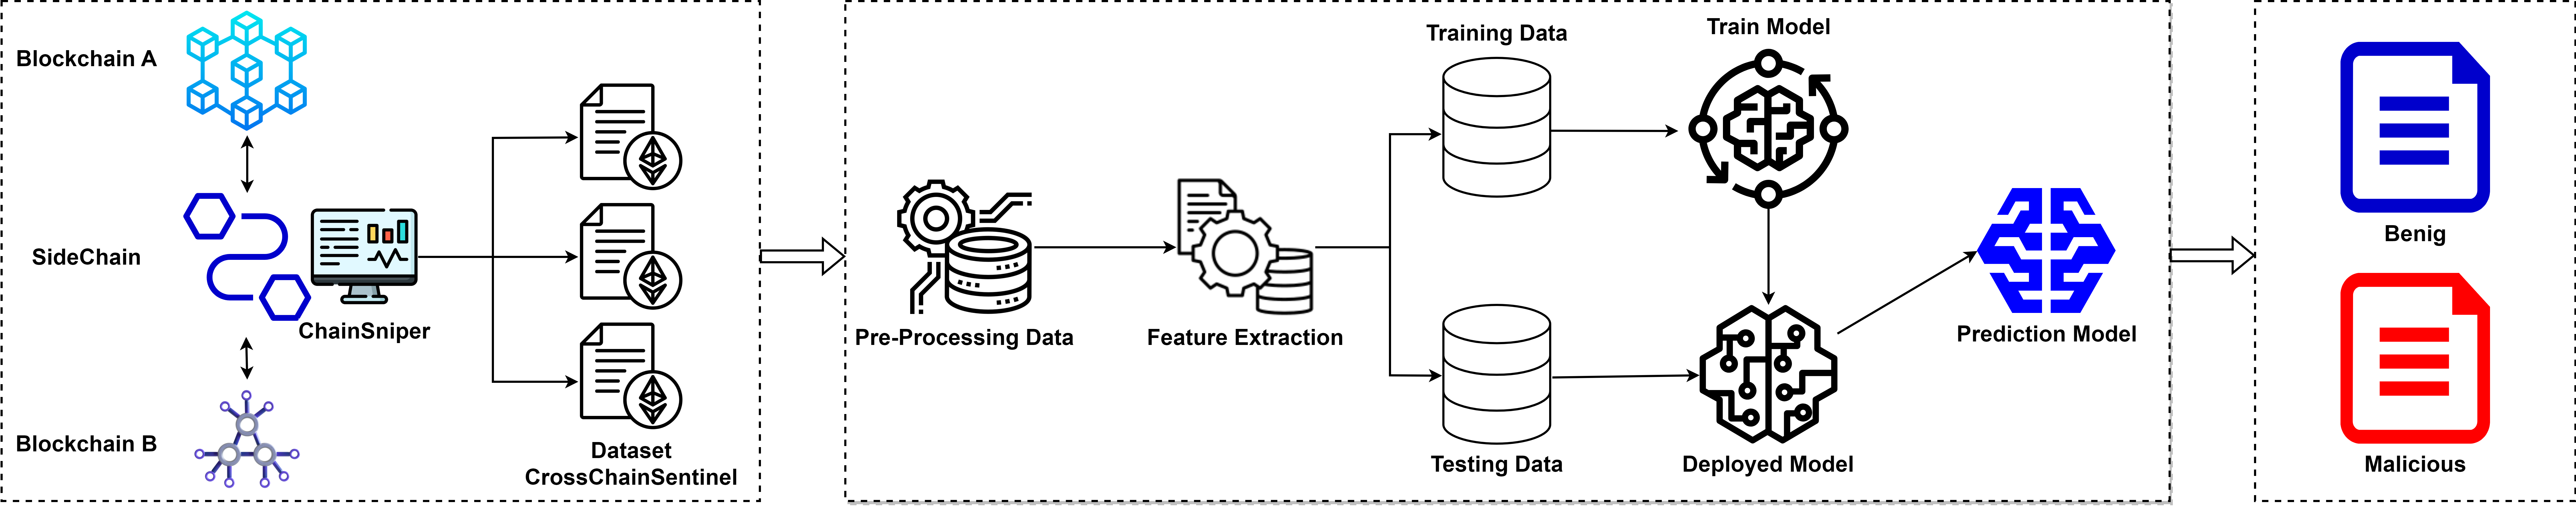
\includegraphics[width=\textwidth]{NewModel.png}
  \Description{The main model presenting the concept of the paper}
\end{figure*}

\vspace{3em}
\section{Proposed Method}
In this section, we first present an elaborate exposition of the ChainSniper system and its constituent components, meticulously outlining their architectural intricacies. Additionally, we expound upon three distinct categories of vulnerabilities that afflict cross-chain smart contracts, providing a comprehensive elucidation of their nature and potential ramifications. Finally, we explicate the meticulous construction process employed in curating the CrossChainSentinel dataset.

\subsection{Main model}
% Mô tả các thành phần trong hệ thống

% The system includes 2 blockchains, transferring data using a bridge which is a side chain, and then transferring data
% Based on the transfer data, capture and structure the dataset
% Then we preprocess the data such as clearing the noise values such as comments, empty spaces.
% label the smart contract into 2 files 1 file is benign and malicious and the other is benign malicious and types of attacks
% then extract the feature to the vector and can be put into the ML phase
% train model, test, and validate
The main model of the ChainSniper has 5 components: 1) Ethereum Sepolia plays a role in Blockchain A 2) Quorum plays a role in Blockchain B 3)The Sidechain transfers data and captures smart contracts, 4) The machine Learning model detects vulnerabilities, and 5) The module classifies the sidechain smart contracts. The system consists of two blockchain networks connected via a sidechain bridge that facilitates data transfer and captures smart contract information. This data is preprocessed and input to machine learning models trained on labeled data to detect malicious contracts. The models are validated to evaluate their performance. Finally, a module leverages the model predictions to classify sidechain smart contracts as either benign or malicious. Figure \ref{newModel} shows the main model:

\subsection{Cross-Chain and Potential vulnerabilities}
\subsubsection{Cross-Chain Networks Overview}
The ChainSniper system enables interoperability between heterogeneous blockchains through a sidechain bridge. The sidechain processes and transfers data between the interconnected networks via a two-way peg mechanism that locks assets on one chain and unlocks equivalent representations on the other using multi-signature contracts. When cross-chain transactions occur, the sidechain nodes log the transaction's data such as contract addresses, timestamps, function calls, parameters, return values, and exceptions. This transaction log is aggregated into a dataset that provides insights into contract behaviors and execution patterns.

\begin{figure*}[h]
  \caption{The sequence diagram of the interchain transfer data}
  \label{transfer}
  \centering
  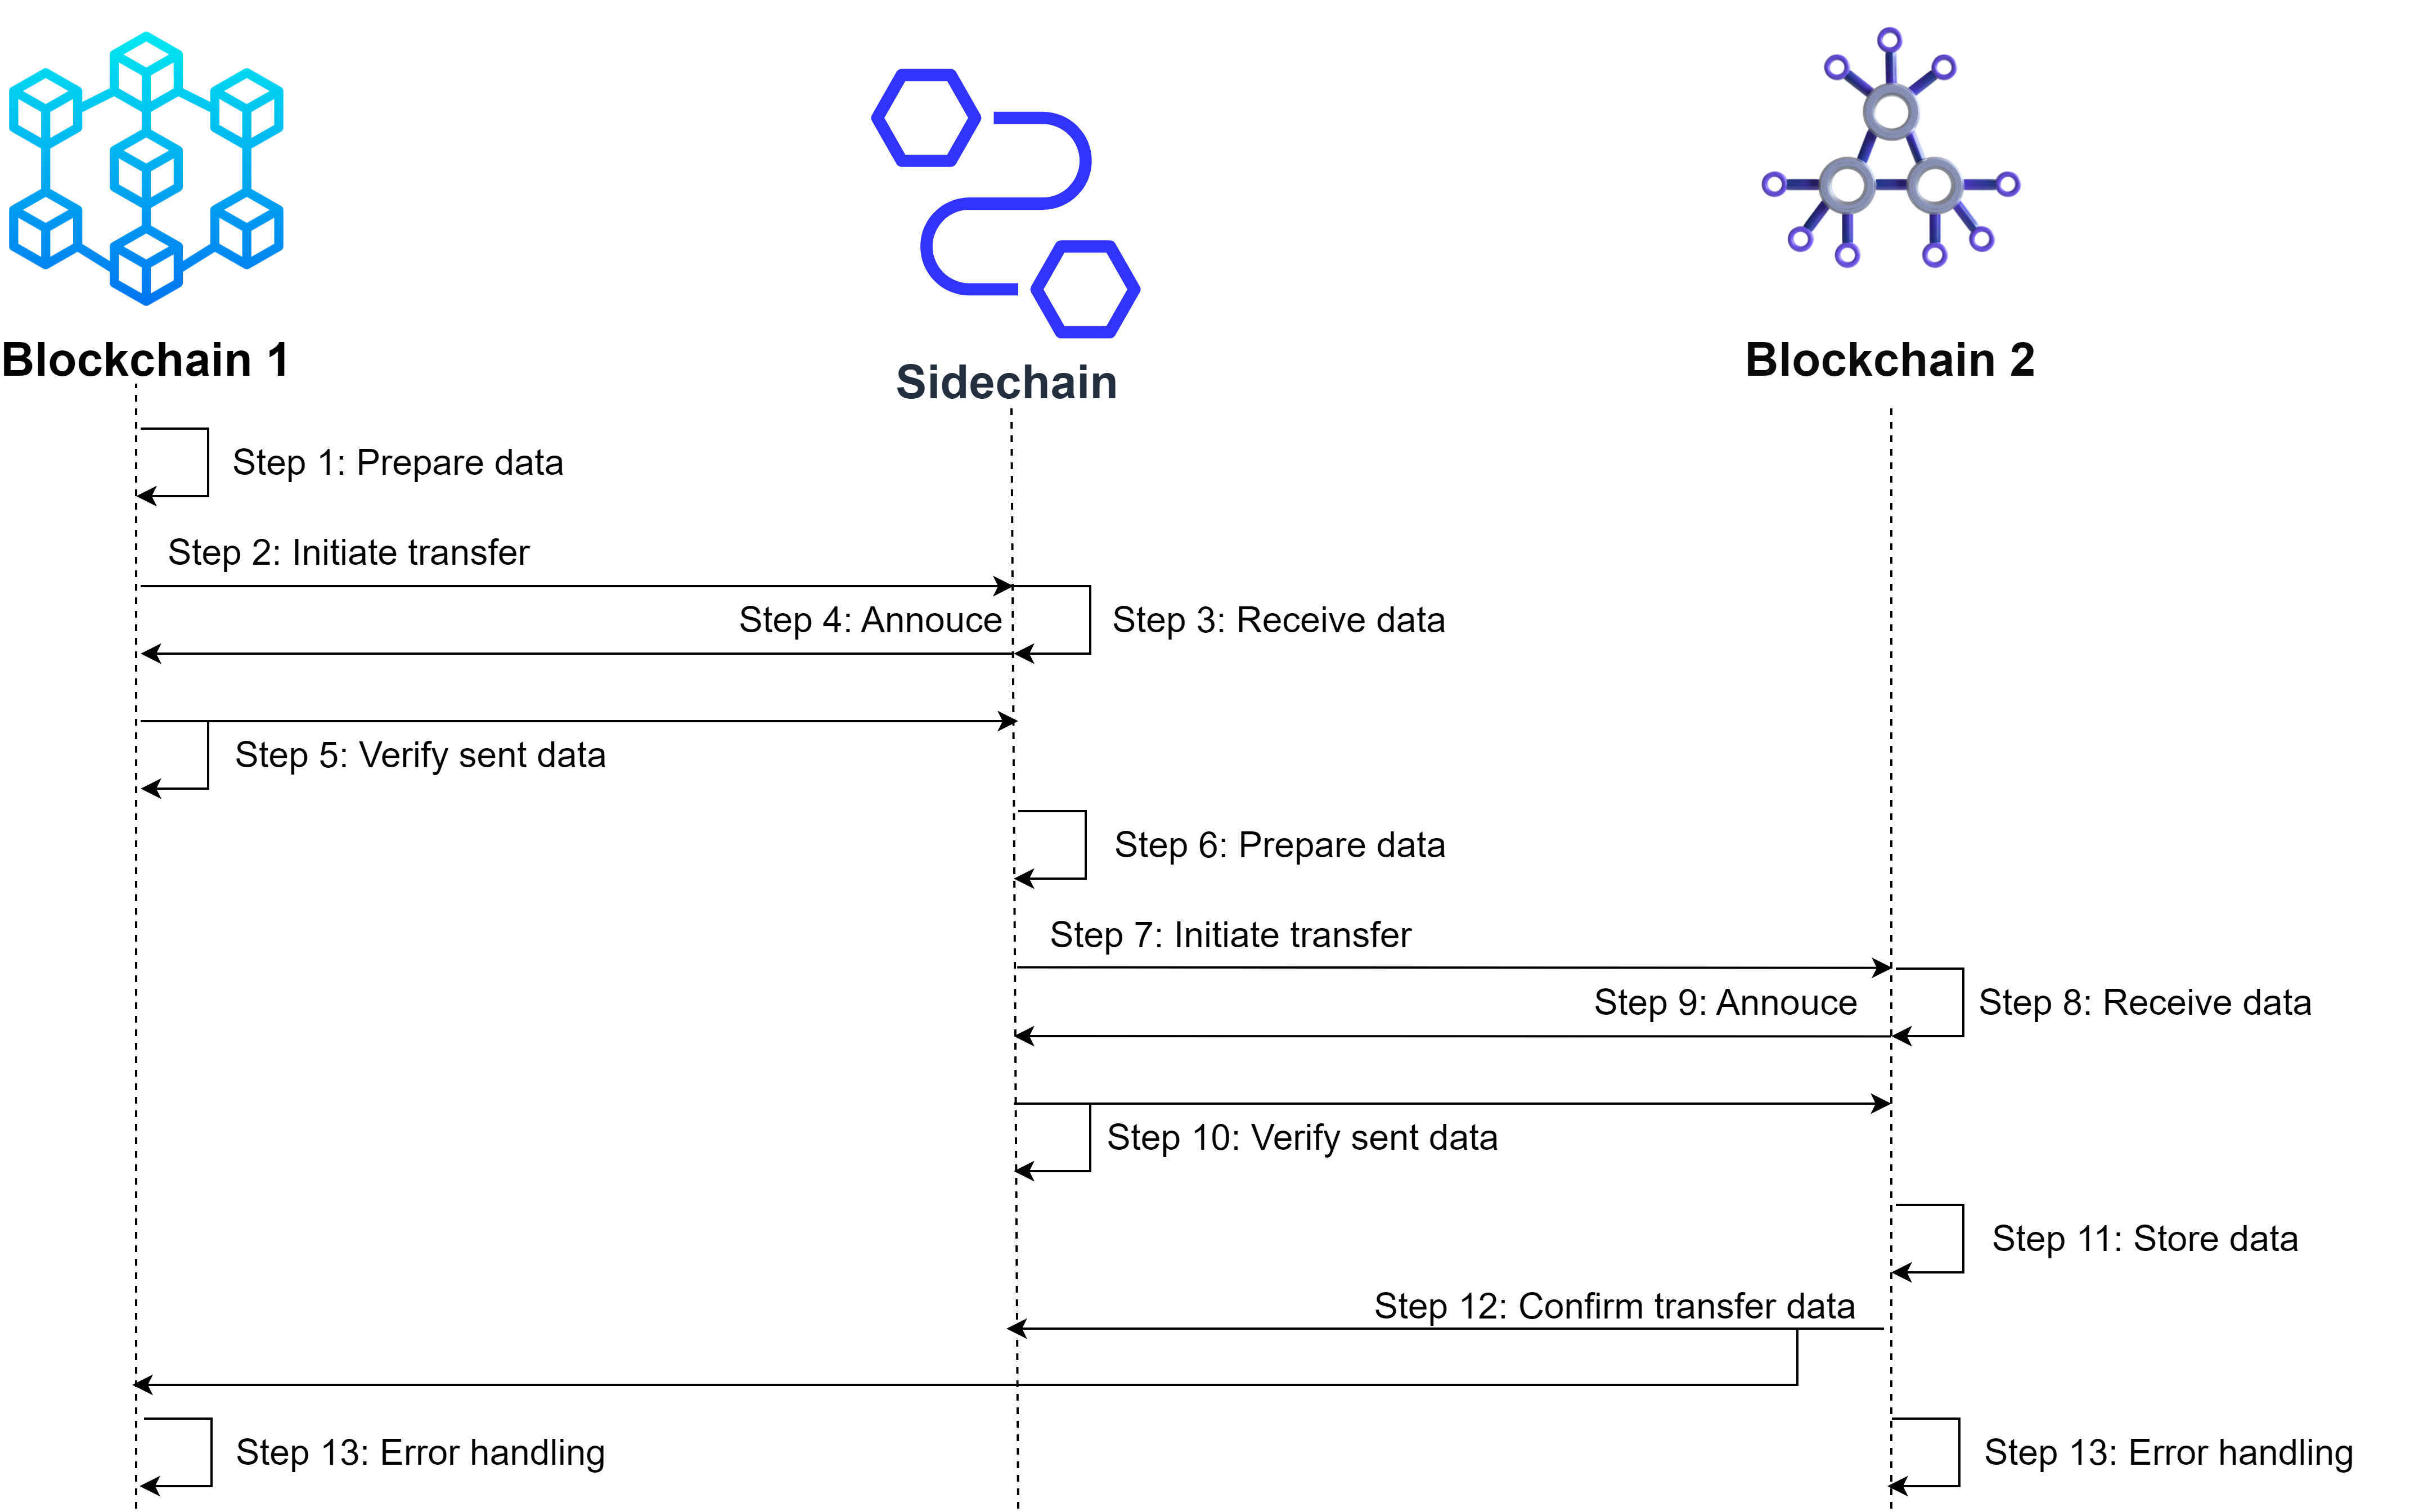
\includegraphics[width=\textwidth]{Step.png}
  \Description{The main step of transfer data}
\end{figure*}

To identify vulnerabilities, static analysis extracts semantic security features from contract source code related to authentication, access control, and encryption. Dynamic analysis also extracts runtime trace features by executing test cases through the sidechain and analyzing the logs. The combined static and dynamic features train machine learning models to accurately detect vulnerable and malicious contracts across interconnected networks. Overall, the sidechain powers seamless interoperability while its logs feed an integrated security pipeline to enhance protection across chains. Figure \ref{transfer} illustrates the main steps to simulate the transfer of data using a sidechain bridge:
\vspace{-0.5em}
\subsubsection{Overflow and Underflow attack in CrossChain}
Overflow and underflow vulnerabilities can arise in CrossChain systems when values exceed or go below the permitted range during math operations, often in smart contracts. This can happen when proper input validation and safe math functions are not used. Attackers exploit these arithmetic bugs to intentionally cause overflow/underflow that lead to unexpected outcomes they can benefit from, like draining excess tokens from a contract. In CrossChain bridges, a lack of protection against these attacks could enable attackers to manipulate asset values as they transfer between chains and steal funds. The algorithm \ref{alg:Overflow/Underflow} simulates the Overflow/Underflow attack:


\begin{algorithm}[h]
\caption{The overflow/underflow attack algorithm}
\label{alg:Overflow/Underflow}
\begin{flushleft}
\SetKwProg{generate}{Function \emph{generate}}{}{end}

\generate{SourceChainContract, DestinationChainContract}{
    sourceBalance = GetBalanceFromSourceChain(SourceChainContract)\\
    amountToSend = MAX\_INT - sourceBalance\\
    \If{CheckTheValueIsValid(amountToSend)}{
        SendFundsToDestinationChain(DestinationChainContract, amountToSend)\\
        destinationBalance = GetBalanceFromDestinationChain(DestinationChainContract)\\
        newBalance = destinationBalance + amountToSend\\
        SetBalanceOnDestinationChain(DestinationChainContract, newBalance)\\
    }
}
\end{flushleft}
\end{algorithm}
\vspace{-1em}
\subsubsection{Reentrancy attack in CrossChain}
Reentrancy vulnerabilities can be exploited in CrossChain systems when contract functions make external calls before updating the state. Attackers can manipulate execution flow to recursively call back into a function before its first invocation completes. For example, in a token transfer function, an attacker could call back in before the sender's balance is updated, allowing them to drain excess tokens. These recursive call attacks can allow hackers to steal funds by repeatedly calling functions before the balance state is updated. The algorithm \ref{alg:Reentrancy} simulates the Reentrancy attack:

\begin{algorithm}[h]
\caption{The Reentrancy attack algorithm}
\label{alg:Reentrancy}
\begin{flushleft}
\SetKwProg{generate}{Function \emph{generate}}{}{end}

\generate{SourceChainContract, DestinationChainContract}{
    LockContract()\\
    CallDestinationChain(DestinationChainContract)\\
    \If{CallbackReceived()}{
        ProcessCallback()\\
        UpdateState()\\
        UnlockContract()\\
    }
}
\end{flushleft}
\end{algorithm}

\subsubsection{Unprotected Ether Withdrawal attack in CrossChain}
CrossChain contracts that hold Ether can be vulnerable to attacks if access controls around withdrawals are not properly implemented. Attackers may exploit unchecked effects or lack of access restrictions in withdrawal functions to arbitrarily drain Ether funds. For example, a withdraw function without validation checks could allow any user to steal Ether by simply calling it. Other risks stem from calling self-destruct or using reentrancy to manipulate Ether transfers. Improper access controls and validations provide avenues for attackers to exploit and steal Ether funds. The algorithm \ref{alg:UnprotectedEtherWithdrawal} simulates the Unprotected Ether Withdrawal attack:

\begin{algorithm}[h]
\caption{Unprotected Ether Withdrawal attack algorithm}
\label{alg:UnprotectedEtherWithdrawal}
\begin{flushleft}
\SetKwProg{generate}{Function \emph{generate}}{}{end}

\generate{SourceChainContract, DestinationChainContract}{
    withdrawalAmount = GetWithdrawalAmount()\\
    \If{CheckTheValueIsValid(withdrawalAmount)}{
        WithdrawEtherFromSourceChain(SourceChainContract, withdrawalAmount)\\
        ReceiveEtherOnDestinationChain(DestinationChainContract, withdrawalAmount)\\
    }
}
\end{flushleft}
\end{algorithm}




\subsection{The CrossChainSentinel Dataset}
\subsubsection{Dataset Construction}
% base on the attack has been mentioned above and the blacklist poly and chainlink, avax and chainlink, ether scan 
% Ref from Smartbugs-wild,  SolidiFi—benchmark
%the dataset have been created base on 15 types of transfer data using cross-chain brigde such as Commos, Avalanche, Chainlink,...
% 300 file - 158 benign - 142 malicious including 42 reentrancy - 48 integer overflow/underflow - 52 unprotected ether withdrawal
% The dataset, named "CrossChainSentinel" - Unveiling Smart Contract Vulnerabilities CrossChain.
A new dataset called CrossChainSentinel\footnote{https://github.com/anhkiet1227/CrossChainSentinel} was created to analyze vulnerabilities in sidechain bridge contracts. The dataset contains 300 smart contract files, with 158 benign and 142 malicious samples. The malicious contracts include 42 with reentrancy vulnerabilities, 48 with integer overflow/underflow bugs, and 52 with unprotected ether withdrawal issues. These were identified using techniques from prior research like Smartbugs-wild\footnote{https://github.com/smartbugs/smartbugs-wild}, SolidiFi-benchmark\footnote{https://github.com/DependableSystemsLab/SolidiFI-benchmark}, and the Blacklists Ethereum address linked to multichain attacks. The cross-chain bridge data was modeled after 15 different real-world providers such as Commos, Avalanche, and Chainlink. The CrossChainSentinel dataset includes common vulnerabilities that can exist when assets are transferred between chains via sidechain contracts. By surfacing these risks in a large labeled dataset, CrossChainSentinel enables more robust auditing, testing, and detection of dangerous flaws in cross-chain bridging mechanisms before mainnet deployment. The diversity of cross-chain sources and vulnerability types makes this dataset well-suited for evaluating tools and models aimed at enhancing cross-chain security.

\subsubsection{Dataset labeling and pre-processing}
% dau tien thuc hien label benign hoac malicious
% cat thanh cac vector
%truyen vao mo hinh
% label the 2 files: 1 labels for benign and malicious smart contracts, 2 labels for benign and malicious smart contracts, including the type of vulnerability they contain
% extract the feature into project is the name of file, commit_id is the information of commit, target with 0 or 1 is benign or malicious, or 0 1 2 3 is benign, mal-reentrancy, mal-overflow, mal-unprotect, func is the structure and content of the file, idx is the number of the file
% base on it change into dimension vector
The data contains two sets of labels. The first set has binary labels indicating whether smart contracts are benign or malicious. The second set has multi-class labels categorizing malicious contracts into more specific vulnerability types: benign, mal-reentrancy, mal-overflow, and mal-unprotect. The data can be extracted into features including the file name (project), commit ID (commitID), label (target), contract structure and content (func), and file number (idx). The benign label is encoded as 0 and the malicious label as 1 for the binary classification set. The multi-class labels are encoded as 0 for benign, 1 for mal-reentrancy, 2 for mal-overflow, and 3 for mal-unprotect. Finally, change the smart contract files to feature vectors and put it into machine learning models to classify vulnerabilities in the contracts.

\subsection{Machine Learning and Deep Learning Models in ChainSniper}
\subsubsection{Machine Learning Models}
We choose machine learning approaches because they allow us to automatically detect vulnerabilities in smart contracts by discerning patterns in the contract code and structure. Compared to manual auditing, machine learning models can analyze contracts more efficiently and consistently. We experiment with several classical machine learning models, including Decision Trees, Random Forests, Support Vector Machines, XGBoost, and Logistic Regression. Owing to their interpretability features, these models enable an understanding of why certain contracts get flagged as vulnerable. Decision trees and random forests build hierarchical rule sets based on code properties to classify contracts. Meanwhile, SVMs find optimal boundaries between vulnerable and benign contracts in feature space. XGBoost further boosts accuracy through an ensemble of weak learners. We extract informative numerical features like function complexity, control flow, and syntax patterns. By training on properly represented data of both positive and negative examples, the models learn robust detectors of security flaws. We apply these techniques in ChainSniper to build an automated scanner for vulnerabilities like Reentrancy, Integer overflows/underflows, and Unprotected Ether Withdrawal. The flexibility of machine learning provides a methodology to detect exploits while avoiding extensive manual effort.

\subsubsection{Deep Learning Models}
We choose deep learning approaches because they can model the intricacies of code logic and dependencies without simplifying manual feature extraction. Techniques like CNNs, RNNs, LSTMs, and Transformer models such as RoBERTa enable end-to-end learning directly from raw smart contract source code to uncover complex syntactic and semantic patterns that characterize vulnerabilities. We experiment with deep neural networks including LSTM-based sequential models that interpret control flows, CNNs that extract local syntax patterns, and Transformer encoders like RoBERTa that provide rich contextual word representations. Owing to their layered hierarchical processing, these networks automatically learn latent relationships between tokens and structure that lead to an understanding of logic indicative of security flaws. For example, the long-range dependencies modeled by LSTMs can trace information flows in a contract to identify unchecked call issues. RoBERTa’s contextual representations discern nuances between seemingly similar constructs that may or may not be vulnerable. The deep learning interpretable attention layers also facilitate identifying the problematic components detected. We apply these techniques in ChainSniper to build automated scanners that can flag potential Overflows/Underflows, Reentrancy, and Unprotected Ether Withdrawal. Avoiding manual feature engineering, deep neural networks can unlock intrinsic comprehension capabilities surpassing classical ML or human abilities for identifying intricate exploit patterns in smart contracts across different blockchains.

\section{Experiments and Security Analysis}
In this section, we perform a series of meticulous experiments, wherein we instantiate the ChainSniper system within a sidechain environment. Leveraging the power of machine learning and deep learning models, we diligently endeavor to unveil vulnerabilities ingrained within cross-blockchain smart contracts. Moreover, we subject the system to rigorous scrutiny, evaluating its performance through a quartet of metrics, namely Accuracy, Precision, Recall, and F1 Score. Additionally, we meticulously compute the average processing time for each machine learning model employed in the audit of cross-chain smart contracts, meticulously elucidating the temporal characteristics of the auditing process. Finally, we engage in an in-depth discourse on system security, expounding upon our findings and offering insightful commentary within the confines of the security analysis segment.

% with sidechain system use 3 machines running Ubuntu 22.04, 4 core CPU, RAM 8GB, 60 GB hard drive
% with the machine learning phase use 2 machines: machine 1 Ubuntu 22.04 4 core CPU, RAM 8GB, 60 GB hard drive, machine 2 use Google Collab Pro running Ubuntu 20.04, T4 GPU, RAM 12.7GB, 166 GB hard drive
% split the data set 8-2 to train and test
% short define about Accuracy, Precision, Recall, F1 Score
% test with Random Forest, XGBoost, CNN, LSTM, SVM with linear, RBF, polynomial, and sigmoid kernels, Logistic Regression,  Feedforward Neural Network, Roberta
% the best performance is Roberta with ACC 0.967, Pre 0.999, Recall 0.875, F1 score 0.933
% Follow up is Logistic Regression, XGBoost
%With the CrossChain phase, we use Ethereum and Quorum as blockchain A and blockchain B to transfer data through sidechain
\subsection{Experiments and Results}
For the experiments, the sidechain system was implemented on 3 machines running Ubuntu 22.04, each with a 4-core CPU, 8 GB RAM, and 60 GB hard drive. The machine learning experiments utilized 2 machines - machine 1 ran Ubuntu 22.04 on a 4-core CPU with 8 GB RAM and 60 GB storage. Machine 2 used Google Colab Pro with an Ubuntu 20.04 environment, T4 GPU, 12.7 GB RAM, and 166 GB hard drive.

\begin{figure*}[h]
  \caption{The performance of the ChainSniper in detecting cross-chain smart contract vulnerabilities}
  \label{timePer}
  \centering
  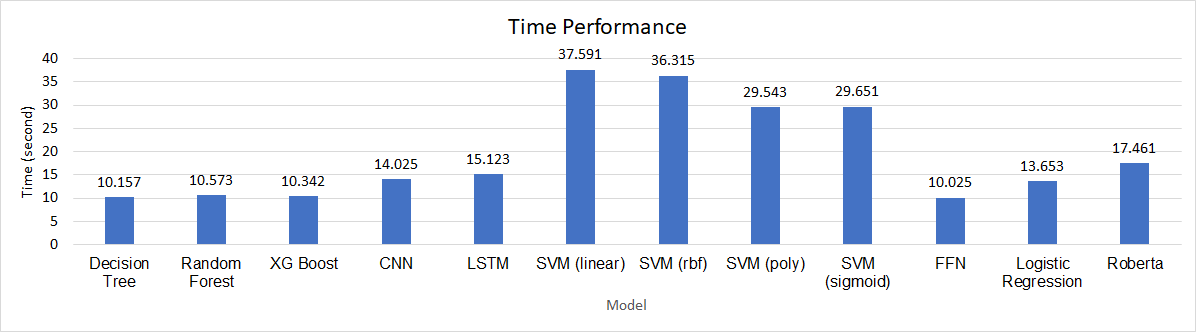
\includegraphics[width=\textwidth]{timePerformance.png}
\end{figure*}

The CrossChain phase utilizes Sepolia Ethereum and Quorum as blockchain A and blockchain B to transfer data through a sidechain connecting the two blockchains. After that, the data was collected and split 80/20 into training and test sets. Accuracy, precision, recall, and F1 score were used as evaluation metrics. The data was tested on Random Forest, XGBoost, CNN, LSTM, SVMs with various kernels, Logistic Regression (LR), Feedforward Neural Network (FFN), and Roberta. Roberta achieved the best performance with an accuracy of 0.967, precision of 0.999, recall of 0.875, and F1 score of 0.933. The next follow-up about performances was Logistic Regression and XGBoost. Overall, models like Roberta performed the best for classifying and identifying vulnerabilities in smart contracts, demonstrating their ability to effectively interpret the semantics and learn predictive patterns from the contract text and metadata. The table \ref{tab:Result} gives information about the result of the experiment:

\begin{table}[H]
    \centering
    \small
    \begin{tabular}{|c|c|c|c|c|}
        \hline
        \textbf{Model} & \textbf{Accuracy} & \textbf{Precision} & \textbf{Recall} & \textbf{F1 Score} \\ \hline
        Decision Tree & 0.598 & 0.723 & 0.618 & 0.666 \\ \hline
        Random Forest & 0.603 & 0.620 & 0.735 & 0.672 \\ \hline
        XGBoost & 0.725 & 0.720 & 0.996 & 0.836 \\ \hline
        CNN & 0.721 & 0.715 & 0.993 & 0.831 \\ \hline
        LSTM & 0.711 & 0.721 & 0.995 & 0.836 \\ \hline
        SVM (linear) & 0.720 & 0.720 & 0.994 & 0.835 \\ \hline
        SVM (rbf) & 0.722 & 0.724 & 0.954 & 0.823 \\ \hline
        SVM (poly) & 0.726 & 0.727 & 0.996 & 0.840 \\ \hline
        SVM (sigmoid) & 0.602 & 0.729 & 0.731 & 0.730 \\ \hline
        FFN & 0.724 & 0.721 & 0.991 & 0.834 \\ \hline
        Logistic Regression & 0.729 &  0.729 & \textbf{0.999} & 0.843 \\ \hline
        \textbf{Roberta} & \textbf{0.967} & \textbf{0.999} & 0.875 & \textbf{0.933} \\ \hline
    \end{tabular}
    \caption{A Comparative Analysis: Performance of Machine Learning Models in Detecting Vulnerabilities within Cross-Chain Smart Contracts}
    \label{tab:Result}
\end{table}

The evaluation tested a variety of machine learning models on a classification task, measuring the inference time per sample in seconds. The fastest model was a simple feedforward neural network (FFN), completing inferences in 10.025 seconds on average. Other very fast models included decision trees (10.157s), random forests (10.573s), and XGBoost (10.342s). The linear support vector machine (SVM) was the slowest, taking 39.591 seconds per inference. In general, the neural network models like CNNs, LSTMs, and Roberta took longer than classical machine learning techniques like SVMs, random forests, and boosted trees. The figure \ref{timePer} gives information about the time performance of the experiment:

\subsection{Security Analysis}
The system was evaluated for its ability to securely detect vulnerabilities and malicious behavior in cross-chain smart contracts. The machine learning models, especially Roberta, were highly effective at classifying and identifying vulnerabilities with accuracy exceeding 96\% and precision nearing 99\%. This demonstrates the system's capability to interpret contract semantics and metadata to learn predictive patterns that pinpoint malicious code. The secure detection capabilities stem from the system's unique cross-chain dataset creation approach that structures raw contract data into robust feature representations. Overall, the results validate the system's security strength for interoperable blockchain networks through its machine-learning models trained on a novel cross-chain dataset. Further security enhancements could involve expanding the diversity and size of training data, tuning additional model hyperparameters, and testing against new types of attacks.

The integration of ChainSniper into the system further supports its security capabilities for detecting vulnerabilities and malicious behavior in cross-chain smart contracts. ChainSniper provides an extra layer of protection through its ability to dynamically analyze real-time dependencies and interactions between contracts across multiple blockchains. By monitoring cross-chain activities as they occur, ChainSniper can identify various behaviors and transaction flows that may be indicative of exploitation attempts. Together, the synergistic combination of ChainSniper's dynamic tracing capabilities and the system's robust machine-learning models enables proactive security monitoring across interoperable blockchain networks. 

\section{Conclusion and Future Works}
% This work proposes and implements a sidechain system to enable data transfer between multiple blockchains for the analysis of smart contract security. A dataset of 300 smart contracts is introduced, with labels indicating benign or three types of vulnerabilities. Machine learning models including deep learning classifiers are developed to detect malicious cross-chain smart contracts. The core innovations are the architecture for inter-blockchain data exchange via sidechains, machine learning modeling for identifying vulnerable contracts, and the ability to detect malicious behavior across interconnected blockchains. Together, the sidechain platform and machine learning techniques represent novel contributions to improving security in multi-blockchain ecosystems.

% Future work should focus on expanding the dataset with more benign and vulnerable smart contract examples to improve model robustness, as well as exploring more advanced deep learning architectures such as transformers and utilizing transfer learning to leverage pre-trained language models for enhanced semantic understanding and malicious contract detection. In the future, our models will be upgraded to automatically detect smart contract vulnerabilities such as reentrancy, integer overflow/underflow, and unprotected ether withdrawal. This will allow proactive identification of weaknesses before deployment, enhancing security and reliability.

This study proposed and implemented a sidechain-based framework, termed ChainSniper, to enable secure inter-blockchain exchange of data for the automated analysis of smart contract security properties. A novel dataset 'CrossChainSentinel' comprising 300 labeled smart contract snippets was introduced. ChainSniper encompassed machine learning models including deep learning classifiers trained on CrossChainSentinel to detect malicious contracts across interconnected blockchain networks. Experimental findings demonstrate the potential of machine learning-driven approaches and sidechain architectures for strengthening smart contract auditing within multi-platform ecosystems and this vulnerability detection system achieved a high accuracy rate of 96\%.

Going forward, avenues for improvement include enlarging CrossChainSentinel with additional benign and vulnerable samples. This would enhance model generalization capabilities. Further exploring advanced architectures such as Transformers leveraging transfer learning from pre-trained language models may boost semantic comprehension for vulnerability identification. Ultimately, iterative upgrades to ChainSniper aim to realize fully automated detection of smart contract weaknesses prior to deployment. This would allow proactive auditing to reinforce reliability and security, advancing the maturity of decentralized applications spanning multiple distributed ledger technologies. Combined with continued data augmentation and algorithm optimization, the proposed framework holds promise for comprehensively screening smart contracts to ameliorate exploitation risks within complex blockchain networks.

\begin{acks}
This research is funded by the Faculty of Computer Networks and Communications, University of Information Technology, Vietnam National University Ho Chi Minh City, Vietnam.
\end{acks}

%\printbibliography
\bibliographystyle{plain} % We choose the "plain" reference style
\bibliography{biblography} % Entries are in the refs.bib file

\end{document}
\endinput
%%
%% End of file `sample-sigconf.tex'.
